%
%	Configure LaTeX to produce a PDF presentation using the beamer class
%


% Default is 16:9 widescreen ratio
\documentclass[ignorenonframetext,12pt,aspectratio=169]{beamer}

% For 4:3 ratio use this:
% \documentclass[ignorenonframetext,11pt]{beamer}


%\documentclass[onesided]{article}
%\usepackage{graphicx}
%\usepackage{beamerarticle}

\usepackage{beamerthemesplit}
\usepackage{patchcmd}
\usepackage{tabulary}		% Support longer table cells
\usepackage{booktabs}		% Support better tables
\usepackage[sort&compress]{natbib}
\usepackage{acronym}			% Support acronyms
\usepackage{listings}			% Allow for source code highlighting

\usepackage{framed}			% Allow background color for images
\definecolor{shadecolor}{named}{white}


\usepackage{subfigure}

\let\oldSubtitle\subtitle


% Configure default metadata
%
%	Configure default metadata in case it's missing to avoid errors
%

\def\myauthor{Author}
\def\defaultemail{}
\def\defaultposition{}
\def\defaultdepartment{}
\def\defaultaddress{}
\def\defaultphone{}
\def\defaultfax{}
\def\defaultweb{}
\def\defaultaffiliation{}

\def\mytitle{Title}
\def\subtitle{}
\def\mykeywords{}


\def\bibliostyle{plain}
% \def\bibliocommand{}

\def\myrecipient{}

% Overwrite with your own if desired
%\input{ftp-metadata}




\AtBeginSection[]
{
   \begin{frame}
       \frametitle{Outline}
       \tableofcontents[currentsection,currentsubsection]
   \end{frame}
}


\long\def\citefoot#1{\let\thefootnote\relax\footnotetext{\citet{#1}} }



\usepackage[utf8]{inputenc}
\usepackage{natbib}
\usepackage{graphicx}

\title{Example of an Article Class Document}
\author{John Smith}
\date{August 2019}

%
%	Get ready for the actual document
%

%
% Use default MMD metadata for beamer equivalents
%

\ifx\subtitle\undefined
\else
	\oldSubtitle{\subtitle}
\fi

\ifx\affiliation\undefined
\else
	\institute{\affiliation}
\fi

\ifx\mydate\undefined
	\def\mydate{\today}
\else
	\date{\mydate}
\fi

\ifx\event\undefined
\else
	\date[\mydate]{\mydate~ / \event }
\fi


%\input{mmd-title}

% Show "current/total" slide counter in footer
\title[\mytitle\hspace{2em}\insertframenumber/
\inserttotalframenumber]{\mytitle}


\author{\myauthor}
\addtolength{\parskip}{\baselineskip}

\ifx\theme\undefined
\else
	\usetheme{\theme}
\fi

\begin{document}
\frame{\setlength\parskip{0pt}\titlepage}


\section{Introduction}
There is a theory which states that if ever anyone discovers exactly what the
Universe is for and why it is here, it will instantly disappear and be replaced
by something even more bizarre and inexplicable. There is another theory which
states that this has already happened.

\begin{figure}[h!]
    \centering
    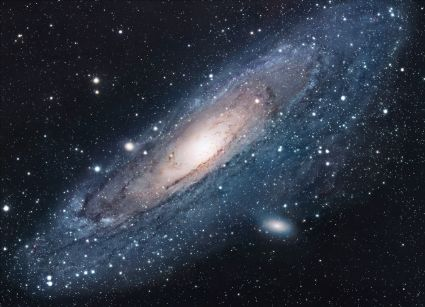
\includegraphics[scale=1.7]{universe}
    \caption{The Universe}
    \label{fig:universe}
\end{figure}

\section{Conclusion}
``I always thought something was fundamentally wrong with the universe''
\citep{adams1995hitchhiker}

\bibliographystyle{plain}
\bibliography{references}

%
%	MultiMarkdown beamer class footer file
%

% Back Matter
\if@mainmatter
\backmatter
\fi

\ifx\bibliocommand\undefined
\else
	\part{Bibliography}
	\begin{frame}[allowframebreaks]
	\frametitle{Bibliography}
	\bibliographystyle{\bibliostyle}
	\def\newblock{}
	\bibliocommand
	\end{frame}
\fi


\end{document}
